\section{Forward Tagger (FT)}


\subsection{Geometry}

The FT detectors are:

\begin{itemize}
	\item a micromegas tracker
	\item an hodoscope
 	\item a calorimeter
\end{itemize}

The three structures are implemented in GEMC using the native perl api script, except for the inner shield (see beamline), which is coming from the CAD engineering mode.

The FT geometry is shown in \F{ftGeometry}.


\begin{figure}
	\centering
	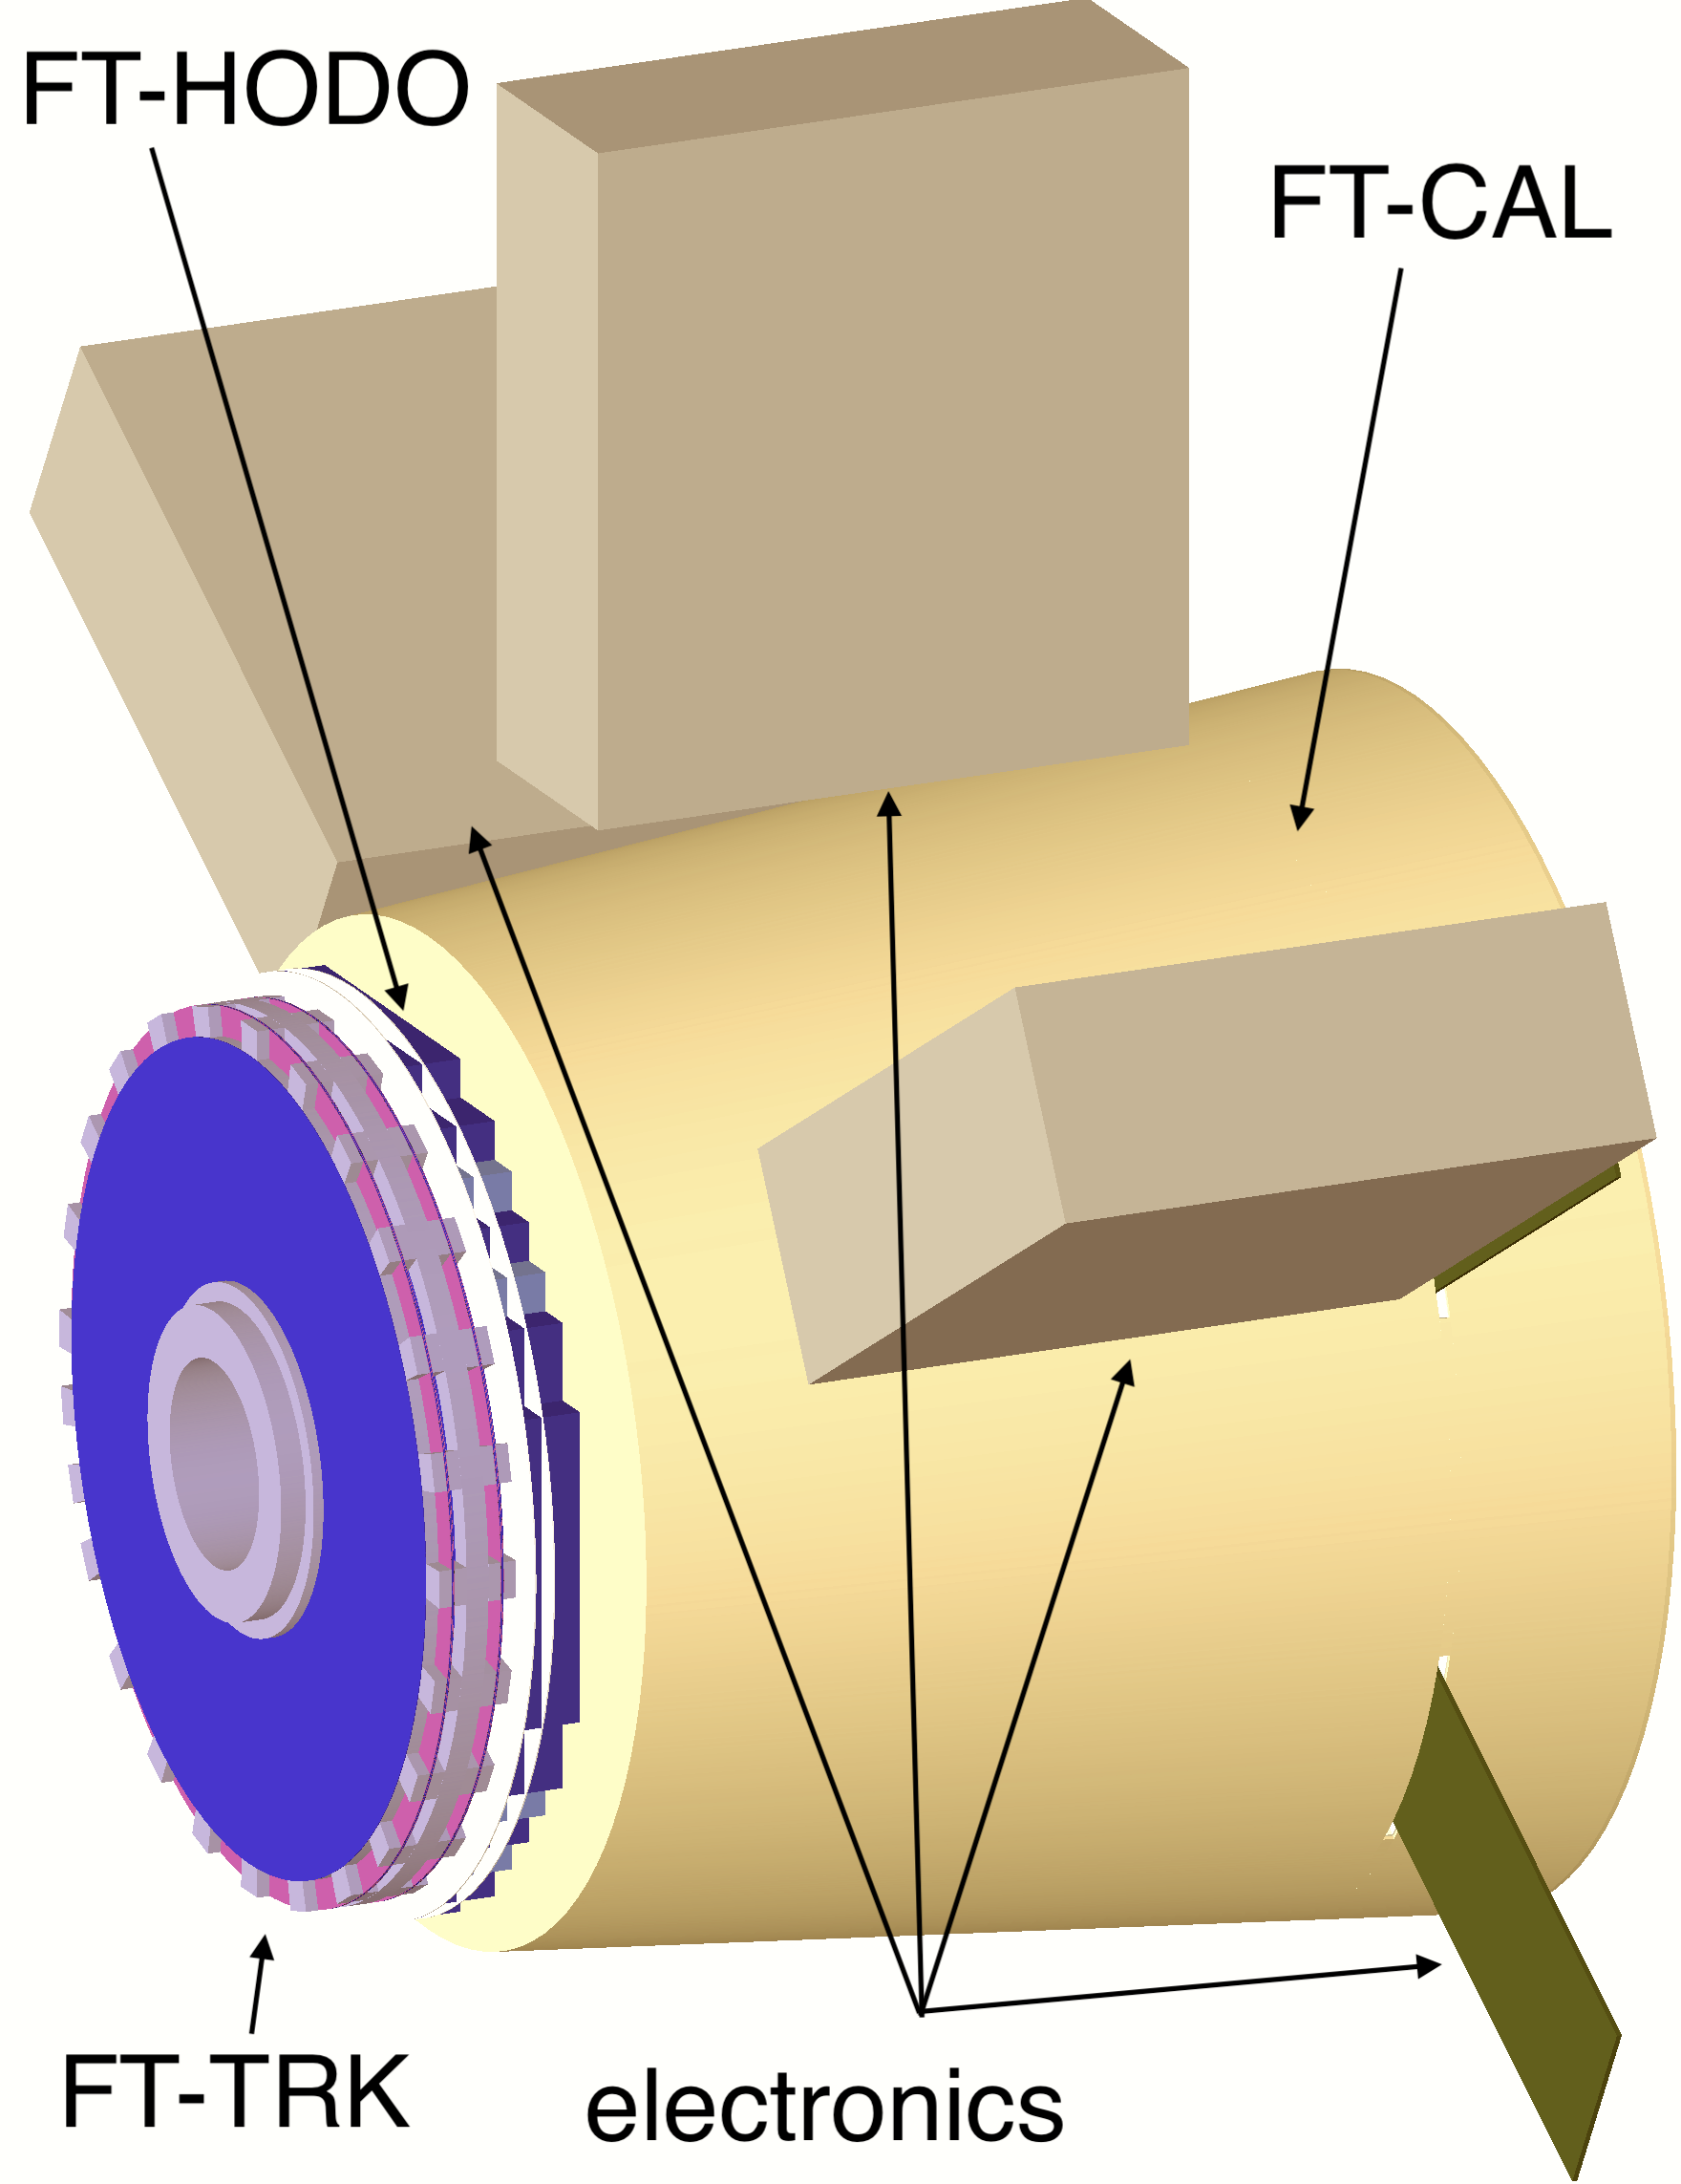
\includegraphics[width=0.95\columnwidth,keepaspectratio]{img/ftGeometry.png}
	\caption{The three detectors in the FT geometry implementation in gemc. The red disks form the micromegas tracker. The hodoscope crystals are the blue boxes,
            while the calorimeter is encompassed in the yellow cone. The grey volumes contains the electronics.}
	\label{fig:ftGeometry}
\end{figure}




\subsubsection{Geometry Git Location}
The github location of the gemc perl api script is \url{https://github.com/gemc/detectors/tree/master/clas12/ft}.


\subsection{Digitization}

\subsubsection{ADC}
For FTCal hits, the energy deposited is converted first to the charge produced at the end of the electronics chain composed by the photosensor (APD) and pre-amplifier, and then to adc. The first conversion is based on the measured charge for cosmic rays that deposit a known energy in the crystals, while the second conversion is based on the FADC conversion factor. A smearing on the final adc values is added, accounting for the Poisson distribution of photo-electrons produced by the photosensor, the Gaussian noise of the photosensor and of the preamplifier. All parameters, number of photo-electrons per MeV of energy deposited, RMS of the APD noise and of the preamplifier input noise, have been tuned to experimental data.

The same approach is adopted to process FTHodo hits, in which the deposited energy is first convereted to charge and then to adc. The smearing in this case accounts only for the Poisson distribution of the measured number of photo-electrons, which dominates over other sources because of the relatively small number of photo-electrons per MeV of energy deposition.

\subsubsection{TDC}
The TDC of FTCal hits is computed from the time of the energy deposition, accounting for the speed of the scintillation light in the crystal and the distance to the photosensor, assuming a known time-to-TDC conversion factor. A Gaussian smearing on the resulting TDC is added based on a fixed RMS derived from the experimental measurements.

Similarly, the TDC of FTHodo hits is derived from the time of a given energy deposition, adding a fixed offset before the conversion from time to TDC and a Gaussian smearing. As in previous cases, all relevant parameters have been tuned to the observed detector response.

\subsubsection{Summary of CCDB Table used}
\paragraph(Calorimeter)
\begin{itemize}
	\item /calibration/ft/ftcal/status
	\item /calibration/ft/ftcal/noise
	\item /calibration/ft/ftcal/charge\_to\_energy
	\item /calibration/ft/ftcal/time\_offsets
	\item /daq/tt/ftcal
\end{itemize}
\paragraph(Hodoscope)
\begin{itemize}
	\item /calibration/ft/fthodo/status
	\item /calibration/ft/fthodo/noise
	\item /calibration/ft/fthodo/charge\_to\_energy
	\item /calibration/ft/fthodo/time\_offsets
	\item /daq/tt/fthodo
\end{itemize}



\subsection{Digitized Bank}
The digitized output bank has $ID=700$, $800$ and $900$ for the FT tracker, the FT hodoscope and the FT calorimeter respectively.
The variables are summarized in Table \ref{tab:ftBank}

\begin{table}[h]
	\begin{center}
		\begin{tabular}{| c | c | c |}
			\hline \hline
			Variable         & Description  & Tag  \\
			\hline
		         & Tracker  &   \\
			\hline
                       sector  &                                     sector   &    1   \\
                        layer  &                                      layer   &    2   \\
                    component  &                                  component   &    3   \\
                          adc  &                                         adc  &    4   \\
			\hline
		         & Hodoscope  &   \\
			\hline
                  sector  &                                     sector   &    1   \\
                        layer  &                                      layer   &    2   \\
                    component  &                                  component   &    3   \\
                          adc  &                                         adc  &    4   \\
                          tdc  &                                         tdc  &    5   \\
			\hline
 		         & Calorimeter  &   \\
			\hline
				        sector  &                                     sector   &    1   \\
				   	      layer  &                                      layer   &    2   \\
				        component  &                                  component   &    3   \\
						        adc  &                                         adc  &    4   \\
						        tdc  &                                         tdc  &    5   \\
			\hline \hline
		\end{tabular}
	\end{center}
	\caption{The digitized FT banks for the tracker, hodoscope and calorimeter}\label{tab:ftBank}
\end{table}

\subsubsection{Time Window}

\subsubsection{Background merging algorithm}

\subsubsection{Process Routine Git Repository Location}
The FT hit process routines are: \url{https://github.com/gemc/source/blob/master/hitprocess/clas12/ft_cal_hitprocess.cc} and
\url{https://github.com/gemc/source/blob/master/hitprocess/clas12/ft_hodo_hitprocess.cc}.
